\documentclass[aspectratio=1610,14pt]{beamer}
\batchmode
%\input{macros.tex}
%\usepackage{xeCJK}
%\setCJKmainfont{STFangsong}
\usepackage{beamerthemesplit}
\usetheme{CambridgeUS}
\useoutertheme{smoothbars}
\usecolortheme{spruce}

\usepackage{xcolor}
\usepackage{amsmath}
\usepackage{amssymb}
\usepackage{graphicx}
\usepackage{graphbox}
\usepackage{eufrak}
\usepackage{color}
\usepackage{slashed}
\usepackage{tcolorbox}

%\def\bch{\begin{CJK}{UTF8}{gbsn}}
%\def\ech{\end{CJK}}
\newcommand{\bch}{}
\newcommand{\ech}{}
\def\bcenter{\begin{center}}
\def\ecenter{\end{center}}
\def\skipline{{\vskip0.1in}}
\def\skiplines{{\vskip0.2in}}
\def\tbox#1{\begin{tcolorbox}#1\end{tcolorbox}}

\newcommand{\field}{\mathscr{F}}

\newcommand{\reals}{\mathbb{R}}
\newcommand{\complexs}{\mathbb{C}}
\newcommand{\ints}{\mathbb{Z}}
%\newcommand{\dim}{\mathrm{dim\ }}
\newcommand{\up}{\uparrow}
\newcommand{\down}{\downarrow}
\newcommand{\del}{\vec \nabla}
\newcommand{\su}{\mathfrak{su}}
\newcommand{\so}{\mathfrak{so}}
\DeclareMathOperator{\tr}{tr}
\DeclareMathOperator{\diag}{diag}
\newcommand{\card}{\mathrm{card \ }}
\newcommand{\mani}{\mathcal{M}}
\newcommand{\lag}{\mathcal{L}}
\newcommand{\ham}{\mathcal{H}}
\def\secpage#1#2{\begin{frame}\bch\bcenter{\bf \Huge #1} \skipline \tbox{#2}\ecenter\ech\end{frame}}
\newcommand{\mat}[1]{\begin{pmatrix}#1\end{pmatrix}}
\newcommand{\unit}[1]{\ {{\rm \ #1}}}
\newcommand{\mev}{\ {\rm MeV}}
\newcommand{\pfrac}[2]{\frac{\partial #1}{\partial #2}}

\newcommand{\bea}{\begin{equation*}\begin{aligned}}
\newcommand{\eea}{\end{aligned}\end{equation*}}

\newcommand{\red}[1]{{\color{red} #1}}
\def\green#1{{\color[rgb]{0.1,0.6,0.3}#1}}
\newcommand{\purple}[1]{{\color{purple} #1}}
\newcommand{\orange}[1]{{\color{orange} #1}}
\newcommand{\blue}[1]{{\color{blue} #1}}
\newtheorem{thm}{定理}[section]
\newtheorem{axm}{公理}[section]
\newtheorem{dfn}{定义}[section]

%\cpic{<尺寸>}{<文件名>}}用于生成居中的图片。
\newcommand{\cpic}[2]{
\begin{center}
\includegraphics[scale=#1]{#2}
\end{center}
}

%\cpicn{<尺寸>}{<文件名>}{<注释>}用于生成居中且带有注释的图片,其label为图片名。
\newcommand{\cpicn}[3]
{
\begin{figure}[h!]
\cpic{#1}{#2}
\caption{#3\label{#2}}
\end{figure}
}


\title{Modern Physics Lab.}
\substitle{E1- HT superconductivity}
\author{H. Gao, Z. Mo, H. Xu, Z. Chen and Z. Fang}
\date{\today}


\begin{document}

\begin{frame}
 
\maketitle
\end{frame}
\begin{frame}{Table of Contents}
\tableofcontents
\end{frame}




\section{The question}
\begin{frame}{A study on the Basic Property of Superconductivity}
Main goals:
\begin{itemize}
\item
$R(T,H=0),\chi(T,H=0)$
\item
The differences between 1st-order PT and 2nd-order PT by comparing $\chi(T,H\not=0)$ for a large $H$.
\end{itemize}
Additional staffs to be explored if time allows:
\begin{itemize}
\item
History dependence of sc.
\item
Other $R(T;H)$ and $\chi(T;H)$ relations near the critical point.
\end{itemize}
\end{frame}

\begin{frame}{Why?}
Let's have a brief review on the theory of superconductivity and phase transition.
\end{frame}


\section{The Theory and the Basic Principles}
\begin{frame}{Electron-phonon Interaction}
\begin{itemize}
\item
QED vertex
$$
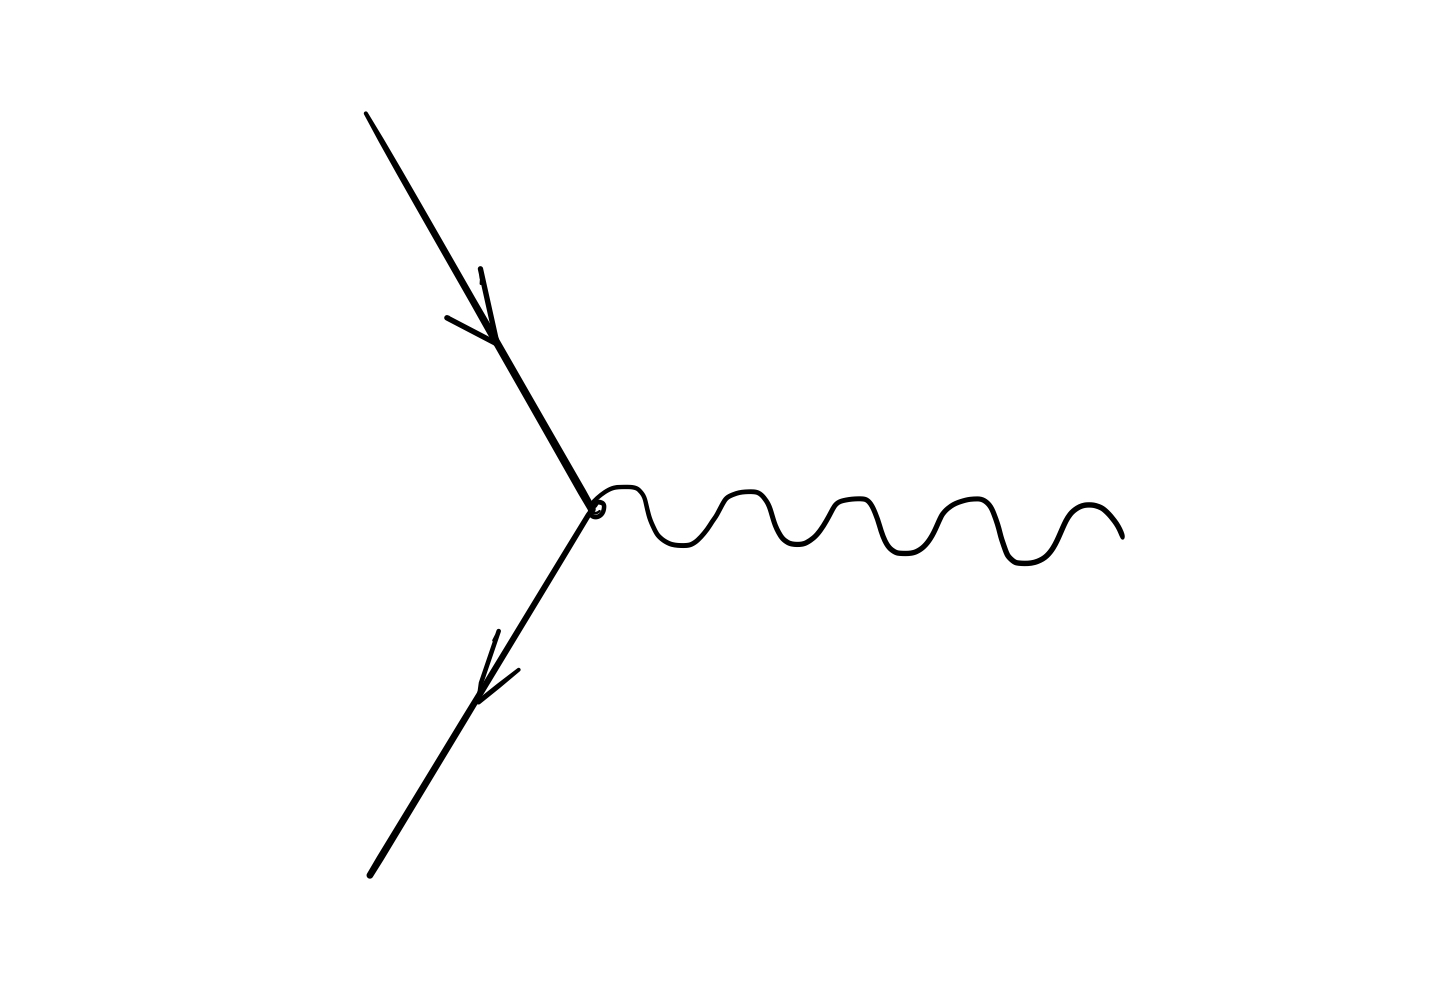
\includegraphics[scale=0.06,align=c]{qed_v} = -ie\gamma^\mu
$$
\item
Electron-phonon interactive vertex
$$
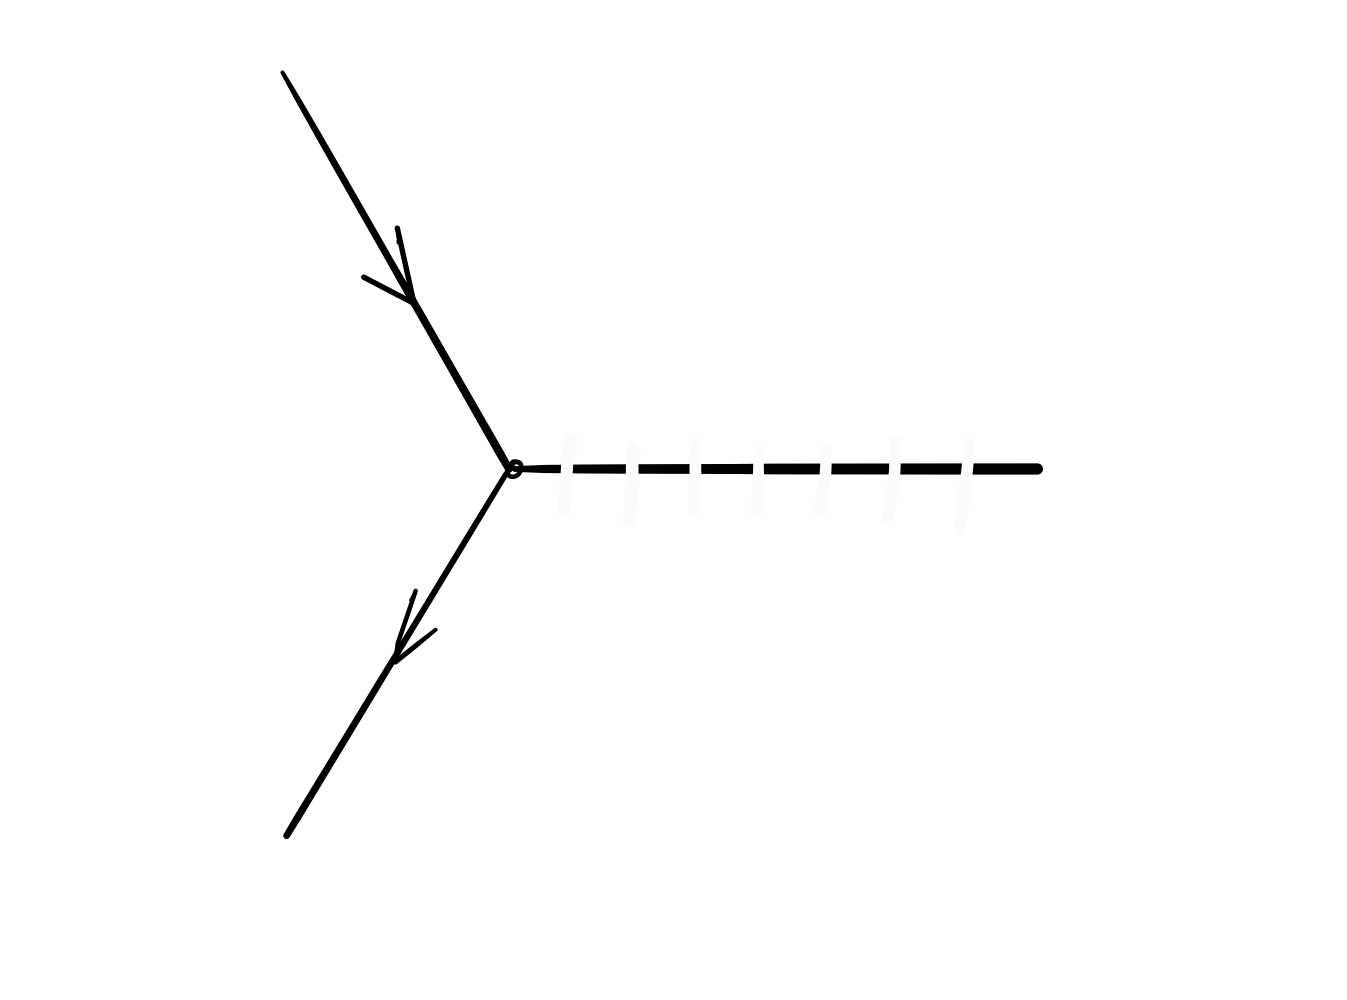
\includegraphics[scale=0.06,align=c]{ep_v} = -ig
$$
\item Similar picture, except\dots
\end{itemize}

\end{frame}


\begin{frame}{Inner Lines in Feynman Diagrams}
\begin{itemize}
\item
In QED, photon is a spin-1 particle (gauge field)
$$\text{photon inner line} =iD^{\mu \nu}(k) = \frac{-ig^{\mu \nu}}{k^2 + i\epsilon}$$
Repulsive force $D^{00} < 0$.
\item
Phonon: a spin-0 particle (abelian real scalar field)
$$\text{phonon inner line} =iD(k) = \frac{i}{k^2 -m^*(k)^2 + i\epsilon}$$
$D>0$, attractive force, results in {\bf electron bound state}, i.e. Cooper pair.
\item
See, for example, Zee, \emph{QFT nut}, Altland, \emph{cond-mat field theory}.
\end{itemize}

\end{frame}

\begin{frame}{Broken Symmetry and Phase Transition}
\begin{itemize}
\item
Electron field = Spinor, with $U(1)$ symmetry in its Lagrangian without an external field..
\item
Superconductivity: $U(1)$ symmetry breaking, selecting a particular ground state.
\item
Symmetry breaking is often related to phase transition $\Rightarrow$ Sc is a new TD phase.
\cpic{0.5}{sb}{\tiny *figure taken from Lancaster/Blundell}
\end{itemize}
\end{frame}

\begin{frame}{Criterions for S.C. State}
\begin{itemize}
\item
Zero resistance:
$$
R\sim 0
$$
In lab: a sudden decreasing in $R$, measured by 4-line method, given by $ R = \frac{V_+ - V_-}{2I}$.
\item
Meissner effect: susceptibility $$1+ \chi \sim 0$$
In lab: a sudden increasing in emf output from lock-in amplifier, given by $\varepsilon \sim \chi$.
\end{itemize}
\end{frame}

\begin{frame}{The Behavior near $T_c$}
\begin{itemize}
\item
We'd ask the exact form of $R(T,H)$ and $\chi(T,H)$.
\iten
1st-order PT: the transition is not {\bf continue}.
\item
2nd-order PT: the transition is not {\bf smooth}, we'd like to say, e.g. 
$$
R(T,H=0) \sim (T-T_c)^\beta
$$
$$
1+\chi(T_c,H) \sim H^{\frac{1}{\delta}}, \quad 1+\chi(T,H=0) \sim (T-T_c)^{-\gamma}
$$
\item {\bf Critical exponents }$\beta,\gamma$ and $\delta$ are NOT integer, i.e. non-analytical behavior.

\end{itemize}
\end{frame}


\begin{frame}{Why Study Critical Exponents}
A very fundamental property of PT, but we're largely innocent of.
\begin{itemize}
\item
Everyday phenomenons: vapor.
\item
In AMO and CMP: BEC.
\item
In hep-th: Higgs mechanism.
\item
In hep-ph/nucl-th: studying the critical exponents reflects our knowledge of symmetry and vacuum (e.g. QCD topological nontrivial vacuum leads to a lot of interesting phenomenons such as CME/CSE, and QCD phase diagram is still largely unknown).
\end{itemize}
\end{frame}

\begin{frame}{QCD Phase Diagram and QCD Vacuum}
\begin{itemize}
\item
QCD Phase Diagram: unknown boundary, even don't know whether PT or not.
\cpic{0.17}{qcd_pd}
\item
Non-trivial QCD vacuum, topological transition.
\cpic{0.3}{qcd_vacuum}
\end{itemize}
\end{frame}

\begin{frame}{Theoretic Calculation}
\begin{itemize}
\item
Mean Field method, of equivalently, Landau 2nd-order PT theory
$$
F(m,T) = F_0 + a(T)m^2 + b(T)m^4
$$
giving $\beta = \frac{1}{2}$, dimensional independence. However, we know that PT doesn't occur in $d=1$ and in $d=2$, one can give exactly $\beta= \frac{1}{8}$ from the first principle.
\item
Why MF fails? Fluctuations.
\item
In $d=3$, unable to solve critical exponents exactly. Must find other solution.
\end{itemize}
\end{frame}

\begin{frame}{Renormalization Group (RG)}
\begin{itemize}
\item
Taking fluctuations into our concern by generalizing Landau theory by considering a field $\phi(\vec x)$ in $d$ dimension space
$$
F[\phi] = \int d^d \vec x \ \frac{1}{2}(\del \phi)^2 + \frac{1}{2}m^2 \phi^2 + \frac{1}{4!}\lambda \phi^4.
$$
No term higher than $O(\del ^2)$ ensures locality.
\item
Partition function as a path integral
$$
Z = \int \mathcal{D}\phi e^{-\beta F[\phi]}.
$$
\item
In $d=4$, equivalent to $\phi^4$ theory in quantum field theory after Wick rotation, which is renormalizable. $\beta$ functions for $m^2$ and $\lambda$.
\end{itemize}
\end{frame}

\begin{frame}{RG flows}
The behavior of RG flows near $W_2$ gives critical exponents as a function of $\epsilon$.
\cpic{0.8}{rg}
{\tiny *figure taken from Lancaster/Blundell}
\end{frame}

\begin{frame}{Results from RG as a $\epsilon$ expansion}
\begin{itemize}
\item
However, we live in $d=3$ space.
\item
Consider $d=4-\epsilon$ Euclidean space, RG flows ($\beta$ functions) give, e.g.
$$
\beta = \frac{1}{2} - \frac{\epsilon}{6} + O(\epsilon^2)
$$
\item Then take $\epsilon =1 $ for $d=3$, we have $\beta = \frac{1}{3}$. Experimentally/Numerically on a lattice, $ \beta \approx 0.3264$.
\end{itemize}
\end{frame}


\begin{frame}{We Can Never Know the Exact Answer}
\begin{itemize}
\item
The result is only from $\epsilon$ expansion and in order to get high order corrections, we have to calculate a HUGE number of Feynman diagrams, which is too arduous (and probably not converge).
\item
RG is also known for its mathematically bad reputation.
\item
So measuring the critical exponents from experiment is of great importance from both practical and theoretic aspects. That's why\dots
\end{itemize}
\end{frame}

\iffalse
\begin{frame}{Tech. in Lab: Low Temperature}
\begin{itemize}
\item
Radiation reduction: a single sheet reduces the radiation loss by $\sim \frac{1}{2} $.
\cpic{0.15}{rad_red}

\item
Temp. control and measurement (Pt1000)
\end{itemize}
\end{frame}
\fi


\section{Our Plan}


\begin{frame}{Our Plan}
\begin{enumerate}
\item
A phenomenological study: measuring critical temp. $T_c$ by two methods (resistance and susceptibility) discussed in sect.1.
\item
A study on the dependence of transition temp. $T(H)$ between external magnetic field $H$.
\item A detailed study on S.C. from the prospect of critical exponents (Our question above).
\end{enumerate}

\end{frame}

\begin{frame}{Let's Keep Focus and Don't Be too Ambitious}
\begin{itemize}
\item
We don't plot $R(T,H)$ our for every $(T,H)$ because it's meaningless from theoretic aspect.
\item
What we are interested in are 2nd-order PTs, i.e., $R(T,H=0),\chi(T,H=0)$ and $\chi(T_c,H)$.
\item
Heavily relies on the precision of measuring $T_c$. Therefore we focus on a particular sample and repeat as many time as possible.
\item
Since the critical exponents of PT are known for universality, focusing on a particular sample would't make us lose any generality.
\end{itemize}

\end{frame}

\begin{frame}{Procedures}
\begin{center}
\begin{tabular}{|c|}

\hline
Measuring $R$ and $\chi$ both from HT $\to$ LT and from LT $\to$ HT \\ \hline
\end{tabular}

$\Downarrow$

\begin{tabular}{|c|}
\hline
Fit the value of $T_c$.\\ \hline
\end{tabular}

$\Downarrow$

\begin{tabular}{|c|}
\hline
Precisely control the temp. at $T_c$ and measure $\chi(T_c,H)$.\\ \hline
\end{tabular}

$\Downarrow$

\begin{tabular}{|c|}
\hline
Measuring $\chi(T,H\not= 0)$ to study the difference btw 1st \& 2nd-order PT.\\ \hline
\end{tabular}

$\Downarrow$

\begin{tabular}{|c|}
\hline
Fit our datas for $(T_c,\alpha,\beta,\delta)$  \\ \hline
\end{tabular}
\end{center}
\end{frame}

\begin{frame}{A Simulative Data Processing}
\begin{enumerate}
\item
Set $\beta = 0.5, T_c = 1$, adding a gaussian noise to every point.
%\cpic{0.5}{data}
\item
Naively fitting data points by LS gives $ T_c =0.82 \pm 0.08$, $\beta = 0.4 \pm 0.3$
\cpic{0.5}{fit}
\item Too large uncertainty in $\beta$, a lot of data points needed.

\end{enumerate}

\end{frame}

\begin{frame}{Tables for Data Recording}
\cpicn{0.5}{rdata}{Table for measuring $R(T,H=0)$.}
\cpicn{0.5}{chit}{Table for measuring $\chi(T,H=0)$.}
\end{frame}
\begin{frame}{More Tables}
\cpicn{0.5}{chib}{Table for measuring $\chi(T_c,H)$.}
\cpicn{0.5}{chi1}{Table for measuring $\chi(T,H\not=0)$ for 1st-order PT.}
\end{frame}


\begin{frame}{Thank You for Your Attentions}
\begin{center}
{\LARGE
We hope you are safe and healthy at home.}
\cpic{0.2}{health}
\end{center}
\end{frame}












\end{document}